%% Manuscript for Biomedical Signal Processing and Control (Elsevier).
%% Built on Elsevier's CAS single-column template (cas-sc.cls).
%% BSPC uses numbered citations (Elsevier style #1) -> model1-num-names.bst.
%%
%% Drafting conventions:
%%   \todo{...}      red, something still to write or decide
%%   \pending{...}   red, a number waiting on an experiment (see results/EXPERIMENTS.md)
%%   \citeneeded{..} red, a claim that needs a verified reference from refs.bib
%% Every number in this file must trace to a run in results/EXPERIMENTS.md.

\documentclass[a4paper,fleqn]{cas-sc}

\usepackage[numbers,sort&compress]{natbib}
\usepackage{xcolor}
\usepackage{multirow}
\usepackage{siunitx}
\sisetup{detect-all}

\newcommand{\todo}[1]{\textcolor{red}{[TODO: #1]}}
\newcommand{\pending}[1]{\textcolor{red}{[PENDING: #1]}}
\newcommand{\citeneeded}[1]{\textcolor{red}{[CITE: #1]}}

\begin{document}
\let\WriteBookmarks\relax
\def\floatpagepagefraction{1}
\def\textpagefraction{.001}

\shorttitle{Lightweight multi-disease retinal screening on low-cost edge hardware}
\shortauthors{S. Agarwal and A. Bhat}

\title [mode = title]{Lightweight multi-disease retinal screening on
low-cost edge hardware}

\author[1]{Shalini Agarwal}[orcid=0000-0003-2892-3723]
\cormark[1]
\ead{shaliniagrawal16@gmail.com}
\credit{Conceptualization, Methodology, Software, Investigation, Formal analysis, Data curation, Visualization, Writing -- original draft}

\author[1]{Aruna Bhat}
\ead{aruna.bhat@dtu.ac.in}
\credit{Conceptualization, Supervision, Validation, Writing -- review \& editing}

\affiliation[1]{organization={Department of Computer Science \& Engineering, Delhi Technological University},
    city={Delhi},
    postcode={110042},
    country={India}}

\cortext[cor1]{Corresponding author}

\begin{abstract}
\textit{Background:} Diabetic retinopathy (DR), glaucoma, cataract and
age-related macular degeneration cause most avoidable vision loss, but
specialists and computing infrastructure are scarce where screening is
most needed.
\textit{Methods:} A single MobileNetV3-small network screens five retinal
conditions from one fundus photograph. It was trained on ODIR-5K and
evaluated on a patient-disjoint held-out test set over three seeds, then
deployed with ONNX Runtime, OpenVINO and TensorFlow Lite on an Intel N100
mini PC and a Raspberry Pi~3B. We measured export fidelity, latency,
memory, energy, INT8 quantization, calibration and on-device Grad-CAM.
\textit{Results:} Raising input resolution from $224\times224$ to
$512\times512$ improved mean test AUC from 0.800 to 0.846 and DR AUC by
0.073 (95\% CI 0.047--0.099). Per-eye DR labels added no measurable gain.
Floating-point deployment was lossless: test AUCs matched the reference to
four decimals on both devices. The model needed 8~ms and 222~MB on the
N100, and 0.51~s and 65~MB on the Pi. Naive INT8 quantization cost up to
0.23 AUC and broke calibration for little speed gain. Class weighting
made outputs over-confident. Temperature scaling failed to correct this,
while Platt scaling reduced DR calibration error from 0.163 to 0.027.
On-device Grad-CAM matched the reference, passed randomisation sanity
checks and added 9--27\% latency on the Pi, but never highlighted
microaneurysms.
\textit{Conclusion:} A floating-point model using under 100~MB on a
low-cost single-board computer matches its workstation accuracy for
five-disease screening, provided calibration includes a bias term and
quantization is avoided.
\end{abstract}

% Generated by paper/make_graphical_abstract.py from the result files.
\begin{graphicalabstract}
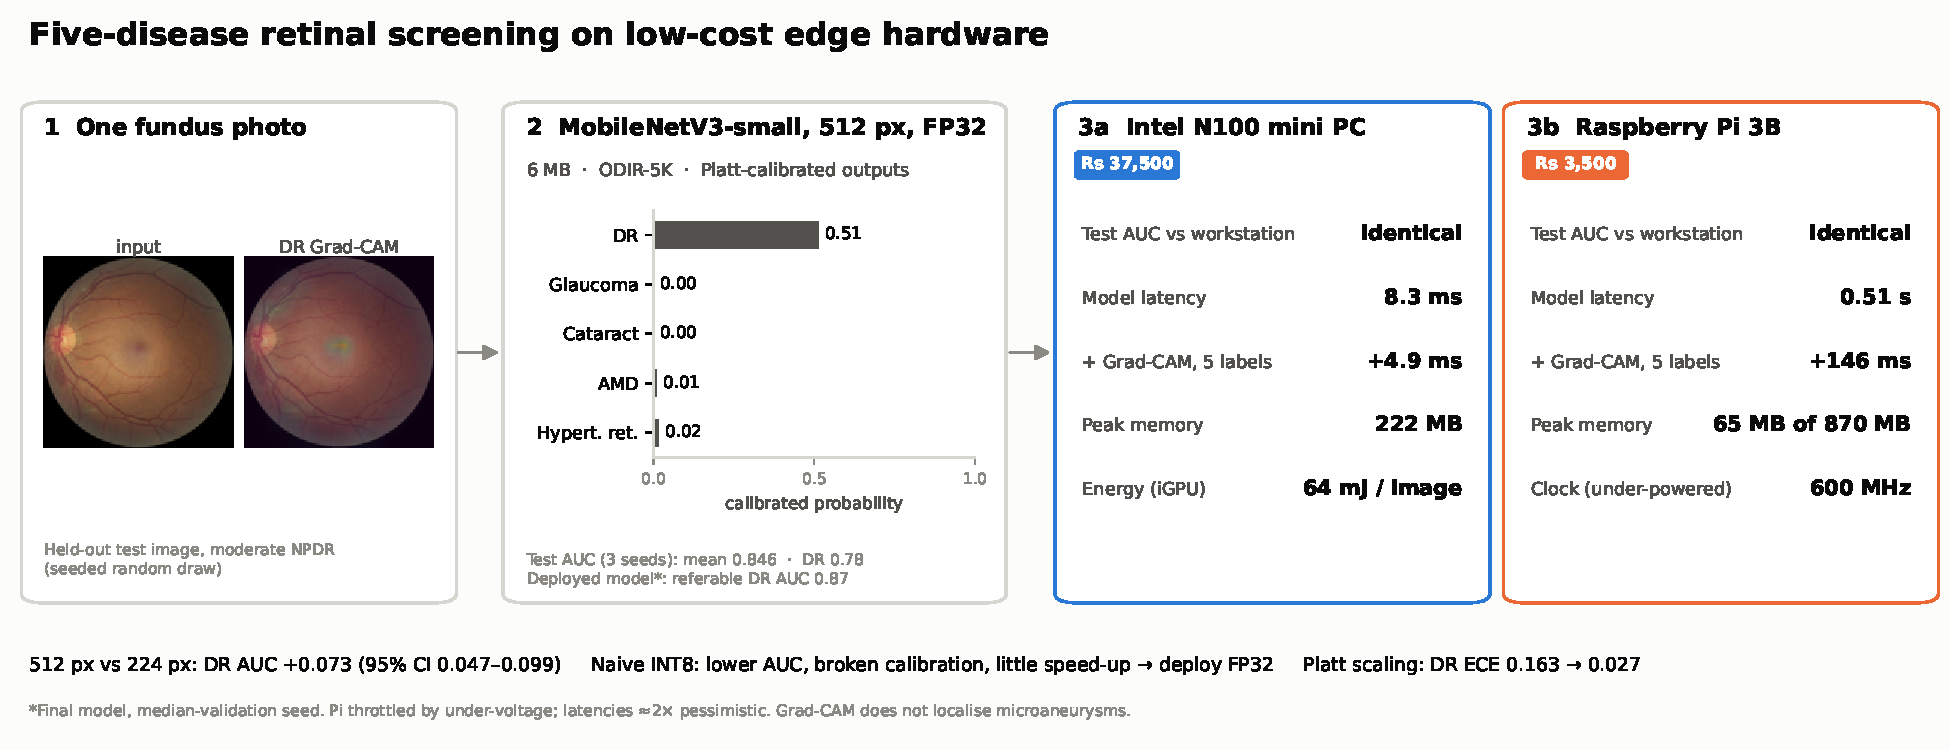
\includegraphics[width=\linewidth]{figs/graphical_abstract.pdf}
\end{graphicalabstract}

% Elsevier: 3-5 bullets, each at most 85 characters including spaces.
\begin{highlights}
\item One lightweight network screens five retinal diseases from a fundus photo
\item FP32 export to an Intel N100 and a Raspberry Pi 3B is lossless
\item 512-pixel input raises held-out DR AUC by 0.07; per-eye labels do not
\item Naive INT8 quantization costs accuracy and breaks calibration
\item Temperature scaling fails under class weighting; Platt scaling works
\end{highlights}

\begin{keywords}
Retinal fundus imaging \sep Multi-label classification \sep Edge computing
\sep Model quantization \sep Diabetic retinopathy \sep Low-resource screening
\end{keywords}

\maketitle

% =====================================================================
\section{Introduction}
\label{sec:intro}

At least 2.2 billion people live with a vision impairment, and in at least
1 billion of them it could have been prevented or has yet to be addressed
\cite{who2019world}. Cataract, glaucoma, age-related macular degeneration
(AMD) and diabetic retinopathy (DR) are among the leading causes of
blindness \cite{steinmetz2021causes}. About 90\% of people with distance
vision impairment live in low- and middle-income countries
\cite{burton2021lancet}, which also have the fewest eye specialists: the
mean density of ophthalmologists is 3.7 per million inhabitants in
low-income countries, against 76.2 per million in high-income countries
\cite{resnikoff2020estimated}. All four conditions, and hypertensive
retinopathy, leave visible signs in a colour fundus photograph, which makes
automated fundus screening an attractive way to extend scarce specialist
capacity.

Deep convolutional networks reach specialist-level accuracy for single
diseases on large curated datasets: an AUC of 0.99 for referable DR
\cite{gulshan2016development}, 0.986 for glaucomatous optic neuropathy
\cite{li2018efficacy} and 0.94--0.96 for AMD \cite{burlina2017automated}.
Three gaps limit their use in low-resource screening. First, most systems
target a single disease, while multi-disease systems rely on hundreds of
thousands of images and server-class models
\cite{ting2017development,cen2021automatic}. Second, performance in
deployment is less reliable than on curated data: seven commercial DR
algorithms evaluated on the same real-world teleretinal images reached
sensitivities between 50.98\% and 85.90\% \cite{lee2021multicenter}, and
image quality, workflow and connectivity constrained a deployed system in
Thai clinics \cite{beede2020human}. Third, most systems assume a
workstation GPU or a cloud connection. Offline on-device screening has
been validated clinically, but only for proprietary single-disease DR
software on smartphones \cite{natarajan2019diagnostic,sosale2020simple}.
Academic edge deployments rarely report whether the deployed model still
matches the trained one, how much memory it needs, or what quantization
costs for each disease (Section~\ref{sec:related}).

This paper measures how much multi-disease screening accuracy survives when
a single lightweight network is deployed on two inexpensive devices: an
Intel N100 mini PC and a Raspberry Pi~3B with less than 1~GB of usable RAM.
The contributions are:
\begin{enumerate}[(1)]
\item a multi-label MobileNetV3-small model that screens five retinal
  conditions (DR, glaucoma, cataract, AMD and hypertensive retinopathy)
  from a single fundus photograph, trained on ODIR-5K and evaluated on a
  patient-disjoint held-out test set with bootstrap confidence intervals;
\item an analysis of why DR performs poorly on ODIR-5K. Interference between
  the five disease heads is not the cause, and input resolution is: on the
  held-out test set, $512\times512$ input raises DR AUC by 0.05--0.07 over
  $224\times224$. Per-eye DR labels, which looked helpful during
  development, gave no measurable gain on the test set;
\item a reproducible edge benchmark of the same model on both devices with
  ONNX Runtime, OpenVINO and TensorFlow Lite. It reports per-label AUC,
  deviation from the reference model, latency distribution, peak memory and, on the N100, energy per
  inference;
\item a negative result for naive INT8 post-training quantization of this
  architecture: it costs accuracy and shifts per-image probabilities,
  without a meaningful speed or memory benefit on either device;
\item an on-device Grad-CAM path that needs no automatic differentiation on
  the device, evaluated with sanity checks, deletion/insertion
  faithfulness and localisation against expert lesion masks, together with
  its cost on both devices;
\item an assessment of confidence calibration on the held-out test set.
  Temperature scaling fails for this model, and Platt scaling works. The
  calibrated outputs survive FP32 deployment exactly, while full-integer
  INT8 breaks them.
\end{enumerate}

% =====================================================================
\section{Related work}
\label{sec:related}

\subsection{Deep learning for retinal disease screening}
Gulshan et~al.\ trained a DR classifier on 128,175 images and reported AUCs
of 0.991 and 0.990 for referable DR on two validation sets
\cite{gulshan2016development}. Ting et~al.\ extended the approach to a
multi-ethnic population and added glaucoma and AMD, using a separate model
for each disease \cite{ting2017development}. Single-disease systems for
glaucoma \cite{li2018efficacy} and AMD \cite{burlina2017automated} report
similar accuracy. In a prospective pivotal trial, the first autonomous DR
system authorised by the FDA reached 87.2\% sensitivity and 90.7\%
specificity \cite{abramoff2018pivotal}, below the retrospective figures.
Two causes of this gap recur in the literature. The first is image and
label quality: adjudicated reference grades together with higher-resolution
input raised the AUC for moderate-or-worse DR from 0.934 to 0.986, and
missed microaneurysms were the most common grading error
\cite{krause2018grader}. A reproduction of the original DR system on public
data with single-grader labels reached only 0.853 on Messidor-2
\cite{voets2019reproduction}. The second cause is the deployment setting
itself \cite{beede2020human,lee2021multicenter}.

\subsection{Multi-label fundus classification}
ODIR-5K provides colour fundus photographs of both eyes for 5,000
patients, with eight diagnostic categories assigned per patient
\cite{li2021benchmark,odir2019challenge}. Work on ODIR has mostly
maximised accuracy with transfer learning, ensembles or bilateral fusion
\cite{islam2019source,wang2020multilabel,gour2021multiclass,he2021multilabel,sun2022efficientnet,wang2024tlccl}.
None of these reports results on low-cost hardware. RFMiD adds 3,200
images from three cameras with 46 conditions \cite{pachade2021retinal}.
Large multi-label platforms reach an AUC of 0.998 across 39 conditions, but
they are trained on about 250,000 images \cite{cen2021automatic}.

\subsection{Lightweight networks and quantization}
MobileNetV3 combines depthwise-separable convolutions, squeeze-and-excitation
(SE) blocks and hard-swish activations, and was designed for mobile CPUs
\cite{howard2019searching,hu2018squeeze,sandler2018mobilenetv2}.
Post-training INT8 quantization usually stays within about 2\% of
floating-point accuracy when weights are quantized per channel
\cite{krishnamoorthi2018quantizing,nagel2021white}, and integer-only
inference underpins TensorFlow Lite \cite{jacob2018quantization}.
Depthwise-separable networks are a known exception: MobileNets often lose
substantial accuracy under post-training quantization, because quantization
error accumulates through the depthwise layers
\cite{yun2021mobilenets,sheng2018quantization}. Data-free equalisation and
bias correction partly recover this loss \cite{nagel2019datafree}.

\subsection{Edge and offline retinal screening}
Offline smartphone AI for referable DR has been validated in community
screening by minimally trained health workers
\cite{natarajan2019diagnostic,sosale2020simple}. Academic edge work mostly
targets DR alone, on a Raspberry Pi~4 \cite{ajithkumar2025efficient}, a
Raspberry Pi or Jetson Nano \cite{kishore2026edge}, or smartphones and
microcontrollers \cite{asare2025deploying,nief2025highly}. Two studies run
multi-disease models on edge devices: ODIR classifiers on a Jetson Nano
\cite{aljbaar2023dcnn}, and an eight-class EfficientNet-B0 with spatial
attention on a Raspberry Pi~5, at about 5~s per image
\cite{thaware2025leveraging}. Energy per image has been measured for
glaucoma classification on an Edge TPU and a Jetson
\cite{rodriguezcorral2024energy}. Reports on quantization disagree. Some
describe INT8 as nearly free \cite{nief2025highly,abushaban2025optimizing},
while a four-class retinal MobileNet study found FP16 better than its
integer variants \cite{farah2026lightweight}.

\subsection{Gap addressed by this work}
None of these edge studies reports, on the target device, whether the
deployed model matches the trained one (AUC and per-image output),
together with peak memory and a per-disease account of quantization cost.
None targets the least capable tier, a Raspberry Pi~3B with 1~GB of RAM and
a 32-bit operating system. We provide these measurements for a
five-condition model on two devices that differ by an order of magnitude in
price and compute.

% =====================================================================
\section{Materials and methods}
\label{sec:methods}

\subsection{Dataset and splits}
We use ODIR-5K \cite{li2021benchmark,odir2019challenge}, obtained as the
widely used preprocessed public mirror, with images cropped and resized to
$512\times512$. It contains 6392 per-eye fundus images from 3358 patients,
annotated with eight patient-level categories. We model five: DR (D),
glaucoma (G), cataract (C), AMD (A) and hypertensive retinopathy (H). The
normal and ``other'' categories are not modelled. Patient-level prevalence
is 1105 (D), 206 (G), 208 (C), 163 (A) and 103 (H) of 3358 patients, so
every label except DR is rare.

All splits are grouped by patient, so both eyes of a patient always fall
in the same partition. A first grouped split (20\%, seed 42) defines a
validation set of 1270 images. This set was used during development to
choose input resolution and DR label definition (Section~\ref{sec:ablation}),
and in the final protocol only to select checkpoints and operating
thresholds. From the remaining images, a second grouped split (20\%, seed
2026) defines a held-out test set that no model was evaluated on until the
final evaluation. The rest is used for training. The final partitions
contain 4097 training images (2148 patients), 1270 validation images (672
patients) and 1025 test images (538 patients). The test set has 285 eyes
with DR under per-eye labels and 62, 62, 42 and 34 positives for
glaucoma, cataract, AMD and hypertensive retinopathy.

\paragraph{Per-eye DR labels.} ODIR-5K assigns its labels per patient, so
an eye without retinopathy inherits a positive DR flag when the fellow eye
is affected. We derive per-eye DR labels from the left- and right-eye
diagnostic keywords supplied with the dataset. Nine keywords denote DR
(mild, moderate and severe non-proliferative DR, proliferative DR, and
generic or suspected DR). Hypertensive and myopic retinopathy are
excluded. These keywords reproduce the patient-level flag exactly for all
1105 positive patients. Of the 2123 images whose patient is DR-positive,
401 (18.9\%) carry no DR keyword for that eye; 250 of them are annotated as
``normal fundus''. The keywords also provide DR severity, which we use for
a referable-DR analysis (moderate non-proliferative DR or worse).

\subsection{Model and training}
The classifier is MobileNetV3-small \cite{howard2019searching}
(\texttt{mobilenetv3\_small\_100} from timm \cite{wightman2019pytorch},
pretrained on ImageNet \cite{deng2009imagenet}) with a five-way sigmoid
output. Training uses AdamW (learning rate $3\times10^{-4}$, weight decay
$10^{-4}$) for 25 epochs, with a two-epoch linear warm-up, cosine decay and
batch size 32. To handle class imbalance we use binary cross-entropy with
a positive weight per label equal to the ratio of negatives to positives in
the training set, clipped to $[1,20]$. Training augmentation consists of
random resized crops (scale 0.8--1.0), horizontal flips, rotations of up to
$\pm 20^\circ$ and colour jitter (brightness and contrast 0.2, saturation
0.1). Evaluation images are only resized and normalised with ImageNet
statistics. We keep the checkpoint with the highest mean validation AUC.

We train three configurations with three random seeds each:
(A)~$512\times512$ input with per-eye DR labels; (B)~$224\times224$ with
the original patient-level labels, the baseline; and (C)~$512\times512$
with patient-level labels, which separates the effect of resolution from
that of the label definition. For deployment we take the configuration-A
seed with the median validation mean AUC, chosen before any test
evaluation.

\subsection{Edge deployment pipeline}
The trained network is exported to ONNX (opset 17) for the N100 and to
TensorFlow Lite for the Raspberry Pi. On each device we re-implement
preprocessing (bilinear resize and ImageNet normalisation) to match the
training pipeline exactly. We verify export fidelity on every evaluation
image by comparing per-image output probabilities with those of the
PyTorch model on the workstation CPU. Runtimes are ONNX Runtime
\cite{onnxruntime} and OpenVINO \cite{openvino} on the N100, and the
TensorFlow Lite (LiteRT) interpreter \cite{litert} on the Pi.

\paragraph{Quantization.} For the N100 we apply OpenVINO/NNCF
\cite{kozlov2021nncf} post-training quantization (mixed preset) calibrated on 300 images drawn
from the \emph{training} split. For the Pi we evaluate TensorFlow Lite
dynamic-range quantization (8-bit weights, float activations) and
full-integer quantization with the same calibration images. No
quantization-aware training or accuracy-aware tuning is applied; this is
deliberately the lowest-effort path a deployer would try first.

\subsection{Confidence calibration}
\label{sec:calib}
Positive-class weighting in the loss inflates predicted probabilities for
rare labels, so raw outputs are not expected to be calibrated. For each
label we fit, by minimising the validation negative log-likelihood, either
a single temperature, $\sigma(z/T)$ \cite{guo2017calibration}, or a Platt
map with scale and bias, $\sigma(az+b)$ \cite{niculescu2005predicting},
where $z$ is the output logit. A positive-class weight $w$ in the loss
shifts the optimal logit by about $\log w$. A bias term can undo that
shift, but a temperature cannot. Both maps are monotonic, so they leave
AUC unchanged, and on the device they cost one or two arithmetic
operations per label. On the test
set we report the expected calibration error (ECE) with 15 equal-width
bins \cite{naeini2015obtaining,guo2017calibration}, an equal-mass
(adaptive) variant, the Brier score and the negative log-likelihood, each
before and after scaling. We obtain confidence intervals for the change in
ECE from 1000 bootstrap resamples of test patients. ECE estimated on
resampled data is biased upward, so we do not report percentile
intervals for ECE itself. We also apply the validation-fitted
temperatures to the probabilities produced on each device, and compare
the raw ECE of FP32 and INT8 variants of the development model.

\subsection{Visual explanations}
\label{sec:gradcam}
We compute Grad-CAM \cite{selvaraju2017gradcam} on the last convolutional
feature map for each of the five outputs. On the edge devices the network
is split in two. The exported backbone returns the feature map, and a small
NumPy implementation computes the classification head and the Grad-CAM
gradient analytically from the exported head weights, so the device needs
no automatic differentiation. We check that the maps match the PyTorch
reference, and evaluate them in three ways. The first is the
parameter-randomisation sanity check \cite{adebayo2018sanity}. The second
is deletion and insertion faithfulness on the held-out test set, against
random and centre-bias baselines. The third is localisation against
pixel-level DR lesion masks from IDRiD \cite{porwal2018indian}.
Deletion and insertion progressively remove (by blurring) or restore the
most salient pixels and track the probability of the target label. We
summarise each curve by its area, over 485 test image--label pairs with
positive labels. IDRiD provides 81 images with expert masks for
microaneurysms, haemorrhages, hard and soft exudates. We obtained it from
a public mirror under its CC~BY~4.0 licence, cropped and resized the
images to $512\times512$ like ODIR, and applied the same transform to the
masks. For localisation we report the pixel-level AUROC of the DR map
against the lesion masks and the pointing game (whether the map maximum
falls inside a lesion). Baselines are a random map, a centred Gaussian
(centre bias) and the glaucoma map of the same image (wrong-class
control). On the devices we time the backbone together with the NumPy
head and Grad-CAM, with the numerical library pinned to one thread. With
default threading, the overhead rose roughly sixteen-fold on the N100,
and one run crashed on the Pi.

\subsection{Hardware and benchmarking protocol}
Table~\ref{tab:hw} summarises the two devices.
\begin{table}[width=.95\linewidth,cols=3,pos=h]
\caption{Edge devices used for benchmarking.}\label{tab:hw}
\begin{tabular*}{\tblwidth}{@{} LLL@{} }
\toprule
 & Intel N100 mini PC & Raspberry Pi 3B \\
\midrule
CPU & 4-core x86-64, up to 3.4 GHz & 4-core ARM Cortex-A53 (ARMv7 OS), 1.2 GHz \\
Accelerator & Intel UHD iGPU (OpenVINO) & none \\
RAM & 15 GB & 870 MB usable \\
OS / Python & Debian 13, Python 3.13.5 & Raspbian 11, Python 3.9.2 \\
Runtimes & ONNX Runtime 1.30.0, OpenVINO 2026.4.1 & TensorFlow Lite runtime 2.13.0 \\
Price paid (INR) & Rs 37,500 & Rs 3,500 \\
\bottomrule
\end{tabular*}
\end{table}

Each configuration runs in its own process, so that peak resident memory
(RSS) is attributable to it alone. We measure accuracy over all 1270
validation images at batch size~1. We measure model-only latency on one
fixed preprocessed image after warm-up: 50 warm-up and 500 timed runs on
the N100, and 20 warm-up and 200 timed runs on the Pi. We report mean and
95th-percentile latency, along with the mean time for preprocessing (JPEG
decoding and resizing). On the Pi we read the clock frequency and the
firmware throttling flags before and after every configuration.
On the N100 we measure package energy with Intel RAPL over sustained 60~s
loops, three repeats per configuration with a 30~s cool-down, both for
inference alone and end to end. An idle baseline is measured before and
after each pass. The Pi has no on-board energy counter.

\subsection{Evaluation metrics}
We report the area under the ROC curve (AUC) for each label and its
unweighted mean across the five labels. For export fidelity we report the
maximum and mean absolute probability difference from the reference.
Test AUCs are reported as the mean $\pm$ standard deviation over three seeds.
The 95\% confidence intervals come from 2000 bootstrap resamples of test
patients, applied to the seed-averaged AUC, and paired resamples give
intervals for the differences between configurations. For each label we
choose a threshold on the validation set that gives 90\% sensitivity, and
report sensitivity and specificity on the test set at that fixed
threshold. For DR we also report AUC by severity grade against eyes
without DR, and for referable DR (moderate non-proliferative or worse
against the rest).

% =====================================================================
\section{Results}
\label{sec:results}

\subsection{Held-out test performance}
\label{sec:test}
Table~\ref{tab:test} reports the three configurations on the 1025-image
held-out test set.

\begin{table}[width=\linewidth,cols=4,pos=h]
\caption{Held-out test AUC (1025 images, 538 patients): mean $\pm$
s.d.\ over three seeds, with the 95\% patient-bootstrap CI of the
seed-averaged AUC in brackets. (A) $512\times512$, per-eye DR labels;
(B) $224\times224$, patient-level DR labels; (C) $512\times512$,
patient-level DR labels.}\label{tab:test}
\begin{tabular*}{\tblwidth}{@{} LCCC@{} }
\toprule
Label & A: 512, per-eye & B: 224, patient & C: 512, patient \\
\midrule
DR (per-eye labels) & $0.780\pm0.032$ [0.747, 0.812] & $0.708\pm0.028$ [0.670, 0.742] & $0.775\pm0.031$ [0.741, 0.806] \\
DR (patient labels) & $0.752\pm0.023$ [0.716, 0.786] & $0.698\pm0.024$ [0.661, 0.735] & $0.755\pm0.019$ [0.720, 0.790] \\
Glaucoma & $0.889\pm0.012$ [0.822, 0.939] & $0.860\pm0.004$ [0.798, 0.908] & $0.885\pm0.008$ [0.815, 0.937] \\
Cataract & $0.918\pm0.023$ [0.873, 0.955] & $0.905\pm0.015$ [0.850, 0.948] & $0.920\pm0.009$ [0.872, 0.957] \\
AMD & $0.852\pm0.024$ [0.765, 0.924] & $0.841\pm0.022$ [0.735, 0.928] & $0.878\pm0.011$ [0.798, 0.946] \\
Hypertensive ret. & $0.791\pm0.021$ [0.703, 0.871] & $0.694\pm0.038$ [0.609, 0.776] & $0.798\pm0.009$ [0.705, 0.880] \\
Mean of five & $0.846\pm0.017$ & $0.800\pm0.018$ & $0.847\pm0.004$ \\
\bottomrule
\end{tabular*}
\end{table}

Higher resolution is the effect that holds on unseen data. Configuration
A exceeds the $224\times224$ baseline B for DR by 0.073 (95\% CI 0.047 to
0.099) under per-eye labels and by 0.053 (0.029 to 0.080) under
patient-level labels. It also exceeds B for hypertensive retinopathy by
0.097 (0.028 to 0.164) and for glaucoma by 0.029 (0.004 to 0.053).
Cataract and AMD do not differ significantly. Per-eye DR labels, by
contrast, bring no measurable benefit at equal resolution: A and C differ
in DR AUC by 0.005 (-0.014 to 0.024), and A is slightly worse for AMD
($-0.027$, $-0.048$ to $-0.007$). Seed-to-seed variation is substantial,
with a standard deviation of 0.02--0.03 for DR.

The deployed model (configuration A, seed with the median validation
score) reaches a test DR AUC of 0.809 under per-eye labels and 0.771
under patient-level labels. Its AUC for referable DR is 0.869. For DR
graded against eyes without DR, its AUC is 0.667 for mild
non-proliferative DR (86 eyes), 0.865 for moderate (156), 0.940 for
severe (25) and 0.966 for proliferative DR (6). For the other labels it
reaches 0.892 (glaucoma), 0.897 (cataract), 0.862 (AMD) and 0.813
(hypertensive retinopathy). This seed happens to be the strongest of the
three on test DR, so the seed means in Table~\ref{tab:test} are the
fairer summary. With thresholds fixed on the validation set at 90\%
sensitivity, test sensitivity and specificity are 0.89/0.47 for DR,
0.89/0.67 for glaucoma, 0.81/0.82 for cataract, 0.81/0.75 for AMD and
1.00/0.29 for hypertensive retinopathy. At such operating points the
model would refer many patients without the disease.

\subsection{Development analysis: why DR underperforms}
\label{sec:ablation}
All numbers in this subsection are on the validation set used for
development. They motivated the choice of resolution and label
definition, which Section~\ref{sec:test} then tests on unseen data. Of the
two effects seen here, only resolution held up on the test set.

At $224\times224$ the joint model reached a DR AUC of 0.695, against 0.82
to 0.94 for the other diseases except hypertensive retinopathy. A
single-task DR model trained with the same recipe reached 0.719. The
difference of 0.025 has a paired bootstrap 95\% CI of $[-0.003, 0.053]$,
so interference between the five heads explains little of the gap.
Table~\ref{tab:ablation} varies input resolution and DR label definition.

\begin{table}[width=\linewidth,cols=6,pos=h]
\caption{DR AUC on the development (validation) set by input resolution and
training label. Two seeds per configuration where shown as
``seed~1 / seed~2''. Mean AUC is over all five labels, with DR scored
against patient-level labels.}\label{tab:ablation}
\begin{tabular*}{\tblwidth}{@{} LLRRRR@{} }
\toprule
Input & DR training label & DR AUC (patient) & DR AUC (per-eye) & Referable DR AUC & Mean AUC \\
\midrule
224 & patient & 0.695 / 0.687 & 0.714 / 0.706 & 0.721 / 0.706 & 0.822 / 0.822 \\
224 & per-eye & 0.700 & 0.717 & 0.721 & 0.827 \\
384 & patient & 0.752 / 0.714 & 0.764 / 0.734 & 0.792 / 0.753 & 0.848 / 0.843 \\
384 & per-eye & 0.734 & 0.763 & 0.793 & 0.843 \\
512 & patient & 0.753 / 0.755 & 0.772 / 0.777 & 0.787 / 0.811 & 0.859 / 0.847 \\
512 & per-eye & 0.769 / 0.783 & 0.803 / 0.813 & 0.841 / 0.849 & 0.856 / 0.861 \\
\bottomrule
\end{tabular*}
\end{table}

Resolution is the main factor. At $512\times512$, DR AUC rises by 0.06 to
0.10 over the $224\times224$ baseline, and the paired bootstrap interval
excludes zero for all four 512-pixel runs. Per-eye labels make no
difference at $224\times224$ and appeared to add about 0.03 at
$512\times512$ in both seed pairs. This gain did not replicate on the
held-out test set (Section~\ref{sec:test}). This is consistent with lesion-scale evidence that small
lesions such as microaneurysms need high resolution to be learned at all
\cite{krause2018grader,sahlsten2019deep}. Higher resolution did not harm
the other labels: hypertensive retinopathy gained most, and glaucoma,
cataract and AMD stayed within seed-to-seed variation. The remaining DR
errors concentrate in mild non-proliferative DR. Against no-DR eyes the
512-pixel per-eye models reached 0.70--0.73 AUC for mild cases (98 eyes),
0.83--0.84 for moderate cases (180 eyes) and 0.95--1.00 for severe
non-proliferative and proliferative cases, which are few (30 severe
non-proliferative eyes in the validation set).


\subsection{Export fidelity and edge performance}
Table~\ref{tab:final_edge} reports the final $512\times512$ model on the
held-out test set (1025 images) on both devices. Latency and memory
depend on the architecture and input size, not on the trained weights, so
Table~\ref{tab:latency} compares $224\times224$ and $512\times512$ inputs
with the same protocol.

\begin{table}[width=\linewidth,cols=8,pos=h]
\caption{Export fidelity of the final $512\times512$ model on the held-out
test set (1025 images). AUCs are per label, with DR scored against per-eye
labels. $|\Delta p|_{\max}$ is the maximum absolute probability difference
from the PyTorch CPU reference.}\label{tab:final_edge}
\begin{tabular*}{\tblwidth}{@{} LLRRRRRR@{} }
\toprule
Device & Runtime & DR & Glaucoma & Cataract & AMD & HR & $|\Delta p|_{\max}$ \\
\midrule
Workstation & PyTorch FP32 (reference) & 0.8093 & 0.8916 & 0.8973 & 0.8616 & 0.8126 & -- \\
N100 & ONNX Runtime FP32, CPU & 0.8093 & 0.8916 & 0.8973 & 0.8616 & 0.8126 & $2.5\times10^{-5}$ \\
N100 & OpenVINO FP32, CPU & 0.8093 & 0.8916 & 0.8973 & 0.8616 & 0.8126 & $1.0\times10^{-5}$ \\
N100 & OpenVINO, iGPU & 0.8083 & 0.8913 & 0.8979 & 0.8625 & 0.8129 & $6.4\times10^{-2}$ \\
Pi 3B$^{\S}$ & TFLite FP32, 4 threads & 0.8093 & 0.8916 & 0.8973 & 0.8616 & 0.8126 & $1.3\times10^{-4}$ \\
\bottomrule
\end{tabular*}
\\[2pt]{\footnotesize $^{\S}$Accuracy does not depend on the clock; see Table~\ref{tab:latency} for the Pi's under-voltage throttling.}
\end{table}

\begin{table}[width=\linewidth,cols=6,pos=h]
\caption{Latency and peak memory at $224\times224$ and $512\times512$
input (FP32, batch size 1). Model-only latency is the mean over timed runs;
end-to-end adds JPEG decoding, resizing and normalisation. The iGPU row was
measured with Intel compute-runtime 26.35 and the patched GPU plugin
(Section~\ref{sec:int8}); CPU rows do not depend on either.}\label{tab:latency}
\begin{tabular*}{\tblwidth}{@{} LLRRRR@{} }
\toprule
Device & Runtime & \multicolumn{2}{c}{Model-only (ms)} & End-to-end (ms) & Peak RSS (MB) \\
 & & 224 & 512 & 224 / 512 & 224 / 512 \\
\midrule
N100 & ONNX Runtime, CPU & 2.06 & 8.29 & 7.3 / 15.9 & 196 / 222 \\
N100 & OpenVINO, CPU & 2.43 & 8.40 & 7.0 / 16.1 & 238 / 257 \\
N100 & OpenVINO, iGPU & 2.74 & 7.02 & 7.1 / 13.8 & 687 / 672 \\
Pi 3B$^{\S}$ & TFLite, 4 threads & 130.4 & 512.5 & 224 / 739 & 48 / 65 \\
Pi 3B$^{\S}$ & TFLite, 1 thread & 172.6 & 856.6 & 263 / 1079 & 44 / 65 \\
\bottomrule
\end{tabular*}
\\[2pt]{\footnotesize $^{\S}$The Pi~3B was under-voltage throttled to 600~MHz throughout (\texttt{get\_throttled}~=~0x50005) because of an inadequate power supply; a correctly powered board runs at 1.2~GHz, so these latencies are roughly twice as long as expected.}
\end{table}

Export of the final model is lossless on every CPU runtime: all five test
AUCs equal the PyTorch reference to four decimals, and per-image
probabilities differ by at most $1.3\times10^{-4}$. The N100's integrated
GPU runs in reduced precision by default. It shifts probabilities by up to
0.064 and AUCs by up to 0.001, so we treat CPU inference as the reference
deployment.

At $512\times512$ the N100 takes 7--8~ms per image for the model and about
14--16~ms end to end. At this resolution the integrated GPU is the fastest
backend, the reverse of the $224\times224$ case. The Pi~3B takes 0.51~s for
the model and about 0.74~s end to end (1.35 images per second), and peaks
at 65~MB. Free memory never fell below 666~MB, so the 870~MB limit is not
binding even at full resolution. Throughout, the Pi reported under-voltage
throttling, with the clock at 600~MHz in every sample during the
four-thread runs. A correctly powered board should therefore be roughly
twice as fast.

\paragraph{Development model at $224\times224$, including INT8.}
Table~\ref{tab:edge} reports the same benchmark for the $224\times224$
development model on the 1270-image validation set, including INT8
variants. The INT8 calibration images were drawn from the original
training split, and 55 of them later fell into the held-out test set.
INT8 is not evaluated on the test set, so no test-set number is affected.

\begin{table}[width=\linewidth,cols=7,pos=h]
\caption{Edge benchmark of the $224\times224$ model on the 1270-image
validation set. Latency is model-only at batch size 1 (mean / 95th
percentile). $|\Delta p|_{\max}$ is the maximum absolute probability
difference from the PyTorch reference. N100 iGPU rows use Intel
compute-runtime 26.35.}\label{tab:edge}
\begin{tabular*}{\tblwidth}{@{} LLRRRRR@{} }
\toprule
Device & Configuration & Mean AUC & DR AUC & $|\Delta p|_{\max}$ & Latency (ms) & RSS (MB) \\
\midrule
\multirow{6}{*}{N100} & ONNX Runtime FP32, CPU & 0.8214 & 0.6947 & $6.3\times10^{-6}$ & 2.06 / 2.05 & 196 \\
 & OpenVINO FP32, CPU & 0.8215 & 0.6947 & $6.2\times10^{-6}$ & 2.43 / 2.44 & 238 \\
 & OpenVINO INT8, CPU & 0.8050 & 0.6673 & 0.92 & 1.97 / 1.98 & 242 \\
 & OpenVINO FP32, iGPU$^{\ddagger}$ & 0.8215 & 0.6944 & 0.059 & 2.74 / 2.78 & 687 \\
 & OpenVINO INT8, iGPU, stock$^{\dagger}$ & 0.6226 & 0.4650 & 0.999 & 3.06 / 3.17 & 716 \\
 & OpenVINO INT8, iGPU$^{\ddagger}$ & 0.8012 & 0.6659 & 0.97 & 3.01 / 3.04 & 711 \\
\midrule
\multirow{6}{*}{Pi 3B$^{\S}$} & TFLite FP32, 4 threads & 0.8215 & 0.6947 & $1.8\times10^{-5}$ & 130.4 / 140.3 & 48 \\
 & TFLite FP32, 1 thread & 0.8214 & 0.6947 & $1.7\times10^{-5}$ & 172.6 / 175.9 & 44 \\
 & TFLite dyn.-range INT8, 4 thr. & 0.8166 & 0.6819 & 0.70 & 165.4 / 195.9 & 39 \\
 & TFLite dyn.-range INT8, 1 thr. & 0.8166 & 0.6818 & 0.70 & 165.1 / 169.3 & 41 \\
 & TFLite full INT8, 4 threads & 0.5926 & 0.4944 & 0.98 & 78.3 / 78.5 & 38 \\
 & TFLite full INT8, 1 thread & 0.5861 & 0.4963 & 0.98 & 151.1 / 162.5 & 38 \\
\bottomrule
\end{tabular*}
\\[2pt]{\footnotesize $^{\dagger}$Unmodified OpenVINO 2026.4.1 GPU plugin,
which mis-indexes 5D quantization ranges and returns NaN for this model
(Section~\ref{sec:int8}).
$^{\ddagger}$OpenVINO 2026.4.1 GPU plugin with our fix for that defect.
The fix does not change FP32 results. $^{\S}$The Pi~3B was under-voltage throttled to 600~MHz throughout (\texttt{get\_throttled}~=~0x50005) because of an inadequate power supply; a correctly powered board runs at 1.2~GHz, so these latencies are roughly twice as long as expected.}
\end{table}

FP32 export is lossless on both devices: on all 1270 images, the outputs
match the reference to within $2\times10^{-5}$ in probability, and the AUCs
are identical to the third decimal. On the N100 the model takes about
2~ms, so preprocessing in Python (about 5~ms) dominates end-to-end time,
which stays well above 100 images per second. The integrated GPU is slower
than the CPU at batch size~1 (2.74 vs 2.06~ms) and uses about three times
the memory.
Replacing the 2022 Debian GPU driver with Intel's current compute runtime
(26.35) shortened iGPU latency by only 9\% (3.02 to 2.75~ms), and left it
unchanged within 1\% at $512\times512$. The gap to the CPU therefore
reflects per-inference dispatch overhead on a very small model, not a
driver fault.
On the Pi~3B the FP32 model takes 130~ms with four threads, plus about
90~ms of preprocessing, and peaks at 48~MB, a small fraction of the 870~MB
available. The Pi reported under-voltage throttling throughout
(\texttt{get\_throttled}=0x50005, 600~MHz), so its latencies are
pessimistic relative to a correctly powered board.

\subsection{INT8 quantization}
\label{sec:int8}
On the N100, naive NNCF INT8 saved under 0.5~ms per image and cost 0.017
mean AUC: DR dropped by 0.027, glaucoma by 0.030 and cataract by 0.024.
Per-image probabilities shifted by up to 0.92, which would also invalidate
any downstream confidence calibration. On the Pi, dynamic-range
quantization cost 0.005 AUC and was \emph{slower} than FP32 with four
threads. Full-integer quantization was 1.7$\times$ faster but collapsed DR
to chance (AUC 0.49). This failure is reproducible on the workstation and
on training images. It persisted when the squeeze-and-excitation pooling
and the most-affected layers were kept in floating point, which indicates
error accumulated across the network rather than a single faulty layer.
On the N100's integrated GPU, the INT8 model collapsed to a mean AUC of
0.62 although the same model reached 0.805 on the CPU. The collapse was
identical with the 2022 Debian GPU driver and with Intel's current
compute runtime, and with 16-bit or 32-bit inference precision, so
neither the driver nor reduced precision causes it. Re-quantizing with
other NNCF presets or with the GPU as target device did not help.
Comparing every intermediate output between CPU and GPU located the fault
in the first depthwise convolution, whose GPU output contained NaN in two
of its sixteen channels on every image tested. A single-layer reproduction
isolated the trigger. NNCF had quantized the depthwise weights with one
range per output channel \emph{and} per kernel column, rather than the
usual one per channel. This layout is valid and the CPU computes it
correctly, but the GPU plugin produced about 5\% error in every channel
and NaN in the last two. The cause is in the plugin's precomputation of
quantization scales, which addressed range tensors with a
four-dimensional offset formula. For five-dimensional ranges this placed
the kernel-column index on the wrong axis and, for the last channels,
read past the end of the range buffer. We corrected the offset
computation and added a regression test. With the corrected plugin the
INT8 model reaches a mean AUC of 0.801 on the iGPU, against 0.805 on the
CPU; the remaining gap reflects the iGPU's default 16-bit arithmetic.
FP32 results are unchanged. At 3.01~ms, however, INT8 on the iGPU is
still slower than the iGPU in its default 16-bit mode (2.74~ms) and the
CPU in FP32 (2.06~ms), and it keeps INT8's loss of accuracy and
calibration. Because the FP32 model already fits
comfortably within the Pi's memory, we recommend FP32 deployment for this
model class.

\subsection{Grad-CAM evaluation}
\paragraph{Fidelity and cost.} On 300 test images and all five labels,
the edge implementation (exported backbone plus NumPy head) reproduced the
PyTorch autograd maps to within $2.3\times10^{-4}$ (ONNX) and
$7.2\times10^{-4}$ (TensorFlow Lite) on a 0--1 scale. The location of the
map maximum was identical in 1499 of 1500 maps. On the devices themselves
the maps stayed within $2.5\times10^{-4}$ (N100) and $3.9\times10^{-4}$
(Pi) of the reference. Producing a DR map, or maps for all five labels,
added 1.7 and 4.9~ms to the N100's 7.5~ms inference (ONNX Runtime). On
the power-capped Pi it added 50 and 146~ms to 547~ms (9\% and 27\%).
Peak memory grew by at most 19~MB, to 81~MB on the Pi.

\paragraph{Sanity check.} Grad-CAM passed the model-parameter
randomisation test \cite{adebayo2018sanity}. Re-initialising only the
classifier dropped the median Spearman correlation with the original maps
to 0.075, below the 0.144 between maps of two unrelated images.
Randomising deeper layers kept it between $-0.045$ and 0.022. Maps of
different labels for the same image were nearly unrelated (median
correlation 0.087), so the maps are class-specific. The data-randomisation
variant was not run.

\paragraph{Faithfulness.} Over all positive test pairs, inserting pixels
in Grad-CAM order recovered the prediction much faster than random or
centre-first order. Insertion AUC was 0.740, against 0.471 (random) and
0.593 (centre), and the margin over centre was 0.147 (95\% CI 0.134 to
0.160). Deletion separated Grad-CAM from random (0.326 vs 0.467) but not
from the centre prior (0.341, $p=0.20$). For DR alone, deletion was
\emph{worse} than the centre prior (0.331 vs 0.294). For cataract,
deletion did not beat random order, which fits a diffuse lens opacity
better than a focal lesion.

\begin{table}[width=\linewidth,cols=6,pos=h]
\caption{Localisation of the DR Grad-CAM against IDRiD expert lesion masks
(81 images; soft exudates present in 40). Pixel AUROC is averaged over
images; the pointing game is the fraction of images whose map maximum lies
inside a lesion of that type.}\label{tab:idrid}
\begin{tabular*}{\tblwidth}{@{} LRRRRR@{} }
\toprule
 & \multicolumn{4}{c}{Pixel AUROC} & Pointing game \\
Lesion type & Grad-CAM (DR) & Random & Centre & Glaucoma map & Grad-CAM / random / centre \\
\midrule
Any lesion & 0.657 & 0.499 & 0.575 & 0.518 & 0.14 / 0.04 / 0.09 \\
Haemorrhages & 0.708 & 0.502 & 0.477 & 0.505 & 0.10 / 0.02 / 0.01 \\
Hard exudates & 0.640 & 0.499 & 0.711 & 0.535 & 0.02 / 0.01 / 0.06 \\
Soft exudates & 0.569 & 0.502 & 0.397 & 0.498 & 0.00 / 0.00 / 0.03 \\
Microaneurysms & 0.622 & 0.499 & 0.580 & 0.515 & 0.01 / 0.00 / 0.00 \\
\bottomrule
\end{tabular*}
\end{table}

\paragraph{Localisation.} On external IDRiD images
(Table~\ref{tab:idrid}), the DR map overlapped expert lesions better than
the random, centre and wrong-class baselines (pixel AUROC 0.657 for any
lesion). It placed 1.7 times more of its mass inside lesions than their
area alone would predict. Agreement was best for haemorrhages. For hard
exudates, which cluster around the macula near the image centre, the
centre prior did better. The map maximum fell on a microaneurysm in only
1 of 81 images. At the network's $16\times16$ feature resolution,
lesions a few pixels wide cannot be pointed at, which is consistent with
saliency benchmarks on small pathologies \cite{saporta2022benchmarking}.
Fig.~\ref{fig:gradcam} shows randomly drawn examples per category,
including failures, and Fig.~\ref{fig:idrid} shows IDRiD overlays. On
ODIR several maps peak at the optic disc or the fovea rather than at
lesions.

\begin{figure}
\centering
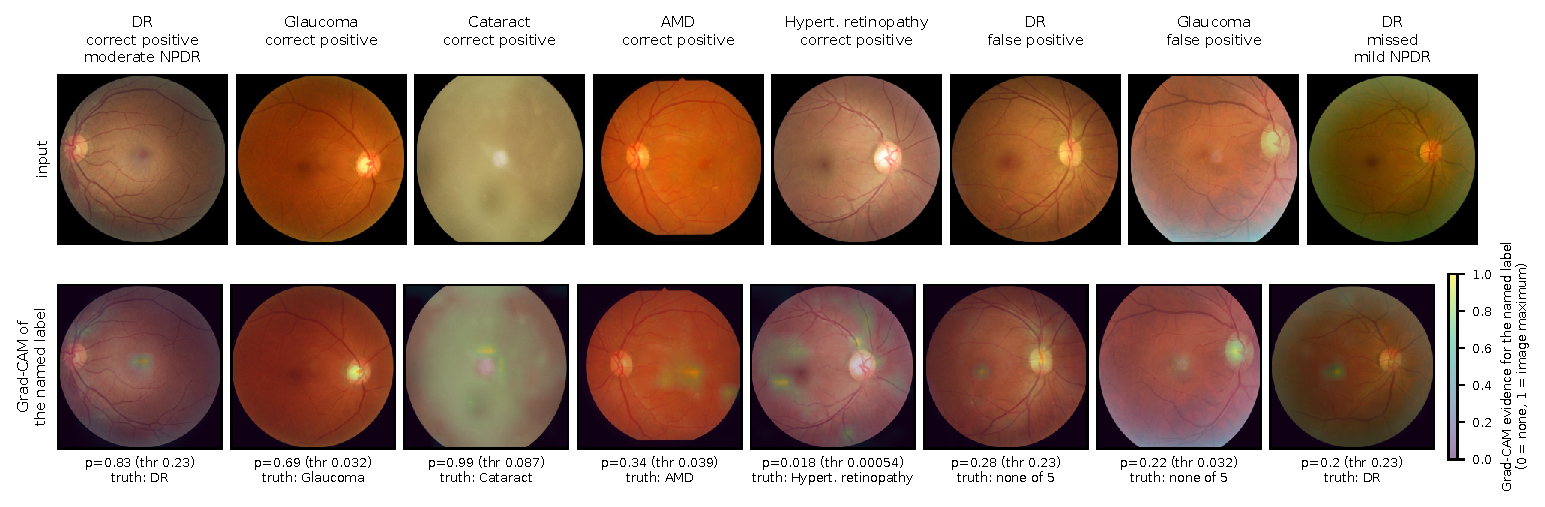
\includegraphics[width=\linewidth]{figs/run010_gradcam_examples.pdf}
\caption{Grad-CAM of the deployed model on held-out test images: one
correct positive per label, a DR and a glaucoma false positive, and a
missed mild non-proliferative DR case. Each example is a seeded random
draw from its category. Colour shows positive evidence for the named
label, scaled to the image maximum. Below each panel: predicted
probability, validation-chosen threshold and ground truth.}\label{fig:gradcam}
\end{figure}

\begin{figure}
\centering
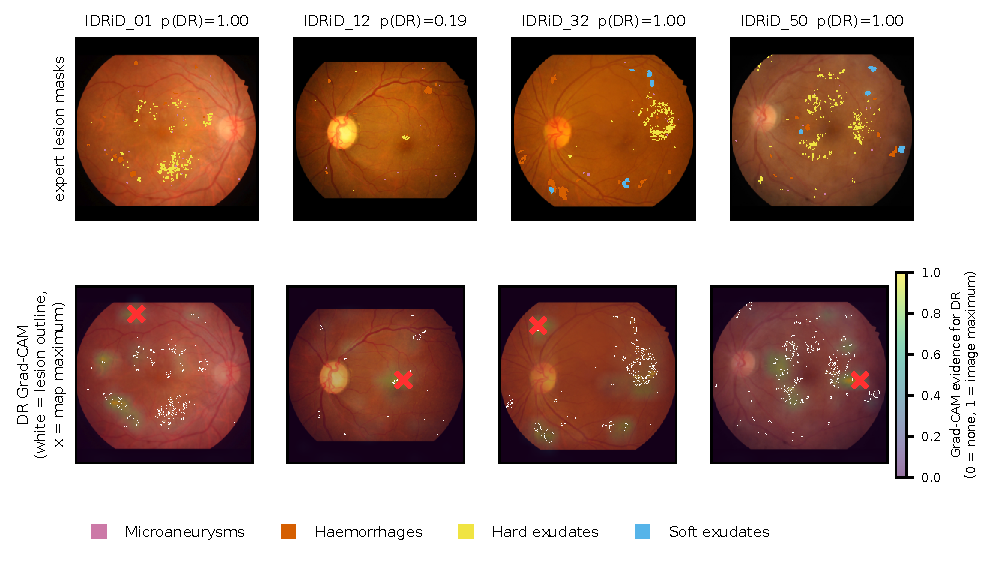
\includegraphics[width=\linewidth]{figs/run010_idrid_overlays.pdf}
\caption{IDRiD images with expert lesion masks (top) and the DR Grad-CAM
with lesion outlines in white and the map maximum marked (bottom).}\label{fig:idrid}
\end{figure}

\subsection{Confidence calibration}
Table~\ref{tab:calib} and Fig.~\ref{fig:reliability} show calibration of
the deployed model on the test set. Raw outputs overestimate disease
probability: the mean predicted probability is 1.5--2.6 times the
prevalence, consistent with the positive-class weights used in training.
Temperature scaling did not help. The temperatures that minimised
validation NLL were all above one (1.12--1.58). They pushed probabilities
towards 0.5 and left ECE unchanged for DR and cataract, and worse for
glaucoma, AMD and hypertensive retinopathy. Platt scaling reduced ECE for
every label, by 0.04 to 0.14 with confidence intervals of the reduction
excluding zero. It brought the mean predicted probability to within 0.01
of the prevalence. The same pattern held for all nine trained models
(ECE after Platt scaling 0.009--0.034, averaged over seeds).

\begin{table}[width=\linewidth,cols=6,pos=h]
\caption{Calibration of the deployed model on the held-out test set. ECE
uses 15 equal-width bins. $\Delta$ is the change in ECE from Platt scaling
with its 95\% patient-bootstrap CI.}\label{tab:calib}
\begin{tabular*}{\tblwidth}{@{} LRRRRL@{} }
\toprule
Label & Prevalence & ECE raw & ECE temperature & ECE Platt & $\Delta$ ECE (95\% CI) \\
\midrule
DR (per-eye) & 0.278 & 0.163 & 0.163 & 0.027 & $-0.136$ [$-0.143$, $-0.094$] \\
Glaucoma & 0.060 & 0.097 & 0.114 & 0.021 & $-0.076$ [$-0.086$, $-0.054$] \\
Cataract & 0.060 & 0.055 & 0.056 & 0.016 & $-0.039$ [$-0.049$, $-0.024$] \\
AMD & 0.041 & 0.058 & 0.084 & 0.012 & $-0.046$ [$-0.055$, $-0.028$] \\
Hypertensive ret. & 0.033 & 0.049 & 0.063 & 0.009 & $-0.040$ [$-0.054$, $-0.018$] \\
\bottomrule
\end{tabular*}
\end{table}

\begin{figure}
\centering
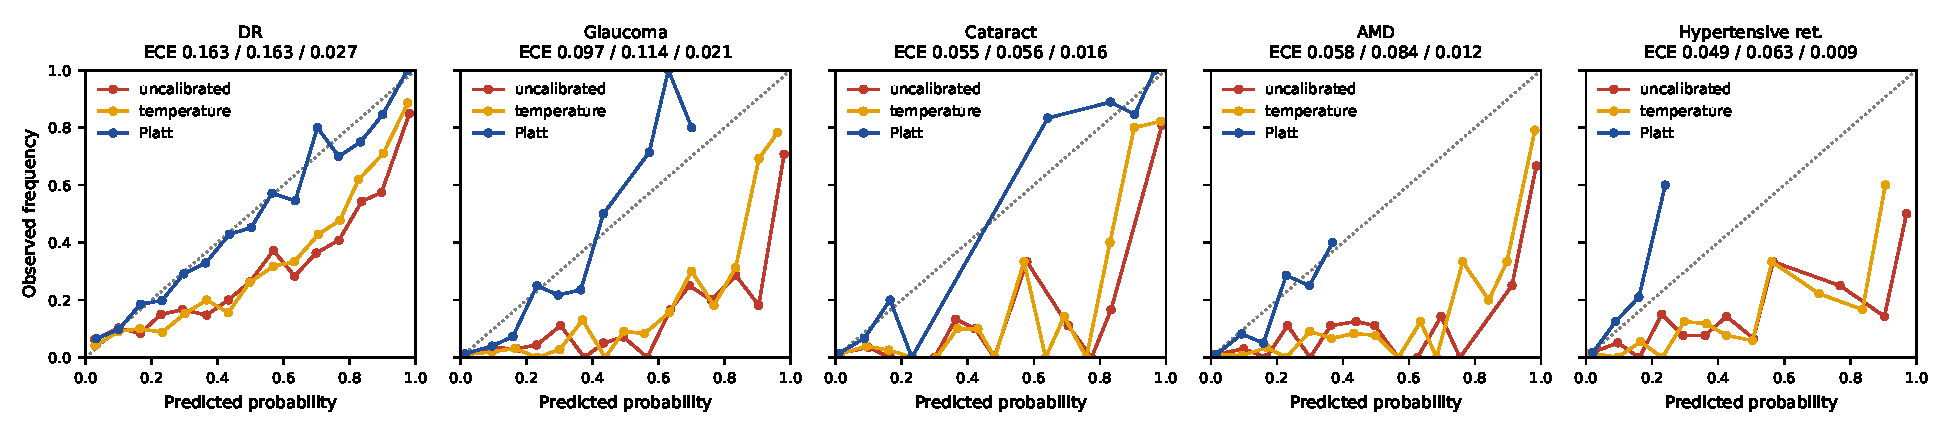
\includegraphics[width=\linewidth]{figs/run011_reliability.pdf}
\caption{Reliability diagrams of the deployed model on the held-out test
set: uncalibrated outputs, temperature scaling and Platt scaling, each
fitted on the validation set. Titles give ECE for the three variants in
that order. Bins with fewer than five images are not drawn.}\label{fig:reliability}
\end{figure}

Calibrated outputs survive deployment. Applying the validation-fitted
Platt maps to the probabilities computed on the N100 CPU runtimes and on
the Pi gives the same ECE as the reference to four decimals for every
label, with calibrated probabilities within $1.4\times10^{-4}$ of it. The
reduced-precision integrated GPU changes DR ECE from 0.027 to 0.028.
Quantization is different. On the $224\times224$ development model, a
Platt map fitted to FP32 outputs and applied to full-integer INT8 outputs
of the same validation images roughly tripled DR ECE (0.025 to 0.080) and
nearly quadrupled cataract ECE (0.014 to 0.051). Dynamic-range INT8
roughly preserved calibration.

\subsection{Energy}
Table~\ref{tab:energy} reports N100 package energy measured with Intel
RAPL over sustained 60~s loops (three repeats, mean $\pm$ s.d.). Idle
package power was 2.6--2.7~W.

\begin{table}[width=\linewidth,cols=6,pos=h]
\caption{N100 energy per inference (package domain, RAPL). Above-idle
subtracts idle package power. Model-only loops repeat inference on one
preprocessed image; end-to-end loops decode and preprocess each image.
Measured with Intel compute-runtime 26.35 and the patched GPU plugin
(Section~\ref{sec:int8}).}\label{tab:energy}
\begin{tabular*}{\tblwidth}{@{} LLRRRR@{} }
\toprule
Input & Runtime & Power (W) & Inferences/s & mJ / inference & mJ above idle \\
\midrule
\multicolumn{6}{@{}l}{\emph{Model-only}} \\
224 & ONNX Runtime, CPU & $11.33\pm0.17$ & $426.5\pm14.4$ & $26.6\pm0.5$ & $20.3\pm0.3$ \\
224 & OpenVINO, CPU & $11.31\pm0.03$ & $343.6\pm1.2$ & $32.9\pm0.0$ & $25.2\pm0.0$ \\
224 & OpenVINO, iGPU & $8.54\pm0.04$ & $370.2\pm0.4$ & $23.1\pm0.1$ & $15.9\pm0.1$ \\
512 & ONNX Runtime, CPU & $11.53\pm0.21$ & $96.0\pm3.8$ & $120.2\pm2.5$ & $93.1\pm1.4$ \\
512 & OpenVINO, CPU & $11.50\pm0.01$ & $89.4\pm0.1$ & $128.6\pm0.1$ & $99.5\pm0.1$ \\
512 & OpenVINO, iGPU & $9.18\pm0.02$ & $143.2\pm0.1$ & $64.1\pm0.2$ & $46.0\pm0.2$ \\
\multicolumn{6}{@{}l}{\emph{End-to-end}} \\
224 & ONNX Runtime, CPU & 9.77 & 137.8 & 70.9 & 51.6 \\
224 & OpenVINO, CPU & 10.74 & 139.7 & 76.9 & 57.9 \\
224 & OpenVINO, iGPU & 8.50 & 119.0 & 71.4 & 49.1 \\
512 & ONNX Runtime, CPU & 11.00 & 59.3 & 185.6 & 141.8 \\
512 & OpenVINO, CPU & 11.09 & 54.0 & 205.3 & 157.2 \\
512 & OpenVINO, iGPU & 9.27 & 73.0 & 126.9 & 91.3 \\
\bottomrule
\end{tabular*}
\\[2pt]{\footnotesize The Raspberry Pi~3B has no on-board energy counter, so its energy was not measured; doing so would need an inline USB power meter, and its under-voltage throttling (Table~\ref{tab:latency}) would also have to be fixed first.}
\end{table}

At $512\times512$ the integrated GPU needs 47--50\% less energy per
inference than either CPU backend (32--38\% less end to end). With the
2022 Debian GPU driver, model-only iGPU energy per inference was 9--21\%
higher (69.6 vs 64.1~mJ at $512\times512$, 28.0 vs 23.1~mJ at
$224\times224$), while end-to-end iGPU figures and all CPU figures changed
by less than 5\%. Under sustained load the N100 settles
at its 10~W long-term power limit, and the package reached 80~$^\circ$C.
Sustained CPU throughput at $512\times512$ (about 10.5~ms per inference)
is therefore lower than the single-shot latency in
Table~\ref{tab:latency} suggests. ONNX Runtime's default thread pool
busy-waits on all four cores, and its power figures include this. Even
end to end at full resolution, one screening image costs about 0.13--0.21~J,
negligible next to the camera and display. The Pi has no on-board energy
counter and was not measured.

% =====================================================================
\section{Discussion}
\label{sec:discussion}

\paragraph{Both tiers are sufficient for throughput.} A screening camera
produces at most a few images per minute. Both devices run the model
far faster than that: the N100 at about 60--140 images per
second end to end, and even the power-capped Pi~3B at 1.35 images per
second at $512\times512$. The cheaper tier is therefore not limited by speed for single-camera
screening, and with 65~MB peak memory at full resolution it is not
limited by memory either. The binding constraint is accuracy.

\paragraph{Quantization is not needed and naive quantization is harmful.}
INT8 is usually justified by memory and speed. Here the FP32 model peaks at
48~MB on the Pi, a small fraction of its memory, and INT8 bought little or
no speed on either device. At the same time, naive post-training
quantization reduced accuracy and shifted per-image probabilities by up to
0.92 (OpenVINO) and 0.98 (TensorFlow Lite full-integer), which would
invalidate any calibrated confidence reported to a health worker. This
agrees with documented post-training quantization difficulties of
depthwise-separable networks \cite{yun2021mobilenets,sheng2018quantization}
and contrasts with edge reports that describe INT8 as nearly free
\cite{nief2025highly}. In our TensorFlow Lite experiments the error was
spread through the network rather than confined to the SE blocks we
inspected. Quantization-aware training or bias-corrected quantization
\cite{jacob2018quantization,nagel2019datafree} may recover accuracy; we did
not test them. Our recommendation is to deploy FP32 for this model class
unless memory forces otherwise.

\paragraph{Calibration needs a bias term.} Weighting the loss by inverse
prevalence is the usual remedy for rare labels, but it leaves every
output biased towards disease. Temperature scaling is often presented as
a near-universal fix \cite{guo2017calibration}, yet it cannot remove a
constant logit offset and made calibration worse here. A two-parameter
Platt map removed the offset at negligible cost. Any screening tool that
shows confidence to a non-specialist and is trained with class
weighting should check for this offset. Because full-integer INT8 shifts
probabilities enough to invalidate a map fitted in floating point, the
calibration step and the deployed numeric format must be validated
together.

\paragraph{DR remains the weakest label.} At $512\times512$ the deployed
model's DR AUC (0.78 averaged over seeds, 0.81 for the deployed seed)
stays below the 0.93--0.99 reported for systems trained on large,
adjudicated datasets \cite{gulshan2016development,krause2018grader}. It
is closer to a reproduction on public data with single-grader labels
\cite{voets2019reproduction}. Referable DR is detected better (AUC 0.87),
and most residual errors are in mild non-proliferative DR, whose
microaneurysms span only a few pixels even at 512 pixels. Per-eye labels
removed an obvious source of label noise (18.9\% of DR-positive images
show no DR in that eye) but did not improve test AUC. Label quality
therefore seems to limit performance less than image detail does. The
preprocessed ODIR-5K images are limited to $512\times512$, so higher input
resolution would require the original images.

\paragraph{Limitations.} All training and testing use a single dataset,
ODIR-5K, whose images were preprocessed by a third party, and there is no
external validation of classification performance. Candidate external
sets are RFMiD \cite{pachade2021retinal} and Messidor
\cite{decenciere2014feedback}; IDRiD \cite{porwal2018indian} was used only
for lesion localisation. Resolution and the DR label definition were
chosen on the validation set, which also selects checkpoints and fits
calibration maps. The held-out test set guards the reported numbers but
not these design choices. Test sets are small for the rarer labels (34--62
positives), as the wide confidence intervals show. The Pi~3B was
power-capped throughout, so its latencies are pessimistic. Each latency
configuration was measured once, and the Pi's energy was not measured.
INT8 was evaluated only on the $224\times224$ development model. Grad-CAM
was evaluated computationally but not in a reader study, and published
evidence cautions that saliency maps can mislead readers
\cite{sayres2019using,saporta2022benchmarking,ghassemi2021false}.

\section{Conclusion}
\label{sec:conclusion}
A single MobileNetV3-small network screened five retinal conditions from
one fundus photograph. It ran on a mini PC and on a Raspberry Pi~3B with
under 1~GB of RAM with no measurable loss of accuracy in floating point.
On the Pi the full $512\times512$ pipeline, including a calibrated output
and a Grad-CAM map, takes under one second per image and stays below
100~MB of memory. Three lessons generalise beyond this model. First,
input resolution mattered more for DR than cleaning the labels. Second,
naive INT8 quantization was not worth its cost, because it degraded both
accuracy and calibration while memory was not a constraint. Third, a
network trained with class weights needs a calibration map with a bias
term before its probabilities can be shown as confidence. The remaining
gaps are clinical: mild DR is poorly detected, Grad-CAM cannot show
microaneurysms, and the model has not been validated on an external
population or with health workers. Those are the next steps.

% =====================================================================
% CRediT statement generated by the template from the \credit{} entries in the front matter.
\printcredits

\section*{Declaration of competing interest}
The authors declare that they have no conflict of interest.

\section*{Data availability}
ODIR-5K \cite{li2021benchmark,odir2019challenge} and IDRiD \cite{porwal2018indian} are publicly available.
The code, export and benchmarking scripts, trained weights and the
patient-level split definitions will be made publicly available in a
GitHub repository upon acceptance. \todo{Add the repository URL once created.}

\section*{Ethical approval}
This article does not contain any studies with human participants or
animals performed by any of the authors. All analyses use publicly
available, de-identified datasets.

\section*{Declaration of generative AI and AI-assisted technologies in the manuscript preparation process}
During the preparation of this work the authors used Claude (Anthropic) to
help write and run analysis and benchmarking code and to draft and edit
the manuscript text. After using this tool, the authors reviewed and edited
the content as needed and take full responsibility for the content of the
published article. \todo{Authors to confirm the wording matches actual use.}

\section*{Funding}
This research did not receive any specific grant from funding agencies in
the public, commercial, or not-for-profit sectors.

\bibliographystyle{model1-num-names}
\bibliography{refs}

\end{document}
